%Version 3 October 2023
% See section 11 of the User Manual for version history
%
%%%%%%%%%%%%%%%%%%%%%%%%%%%%%%%%%%%%%%%%%%%%%%%%%%%%%%%%%%%%%%%%%%%%%%
%%                                                                 %%
%% Please do not use \input{...} to include other tex files.       %%
%% Submit your LaTeX manuscript as one .tex document.              %%
%%                                                                 %%
%% All additional figures and files should be attached             %%
%% separately and not embedded in the \TeX\ document itself.       %%
%%                                                                 %%
%%%%%%%%%%%%%%%%%%%%%%%%%%%%%%%%%%%%%%%%%%%%%%%%%%%%%%%%%%%%%%%%%%%%%
%%\documentclass[referee,sn-basic]{sn-jnl}% referee option is meant for double line spacing

%%=======================================================%%
%% to print line numbers in the margin use lineno option %%
%%=======================================================%%

%%\documentclass[lineno,sn-basic]{sn-jnl}% Basic Springer Nature Reference Style/Chemistry Reference Style

%%======================================================%%
%% to compile with pdflatex/xelatex use pdflatex option %%
%%======================================================%%

%%\documentclass[pdflatex,sn-basic]{sn-jnl}% Basic Springer Nature Reference Style/Chemistry Reference Style


%%Note: the following reference styles support Namedate and Numbered referencing. By default the style follows the most common style. To switch between the options you can add or remove �Numbered� in the optional parenthesis. 
%%The option is available for: sn-basic.bst, sn-vancouver.bst, sn-chicago.bst%  
 
%%\documentclass[sn-nature]{sn-jnl}% Style for submissions to Nature Portfolio journals
%%\documentclass[sn-basic]{sn-jnl}% Basic Springer Nature Reference Style/Chemistry Reference Style
\documentclass[sn-mathphys-num]{sn-jnl}% Math and Physical Sciences Numbered Reference Style 
%%\documentclass[sn-mathphys-ay]{sn-jnl}% Math and Physical Sciences Author Year Reference Style
%%\documentclass[sn-aps]{sn-jnl}% American Physical Society (APS) Reference Style
%%\documentclass[sn-vancouver,Numbered]{sn-jnl}% Vancouver Reference Style
%%\documentclass[sn-apa]{sn-jnl}% APA Reference Style 
%%\documentclass[sn-chicago]{sn-jnl}% Chicago-based Humanities Reference Style

%%%% Standard Packages
%%<additional latex packages if required can be included here>

\usepackage{graphicx}%
\usepackage{multirow}%
\usepackage{amsmath,amssymb,amsfonts}%
\usepackage{amsthm}%
\usepackage{mathrsfs}%
\usepackage[title]{appendix}%
\usepackage{xcolor}%
\usepackage{textcomp}%
\usepackage{manyfoot}%
\usepackage{booktabs}%
\usepackage{algorithm}%
\usepackage{algorithmicx}%
\usepackage{algpseudocode}%
\usepackage{listings}%


%%%%

%%%%%=============================================================================%%%%
%%%%  Remarks: This template is provided to aid authors with the preparation
%%%%  of original research articles intended for submission to journals published 
%%%%  by Springer Nature. The guidance has been prepared in partnership with 
%%%%  production teams to conform to Springer Nature technical requirements. 
%%%%  Editorial and presentation requirements differ among journal portfolios and 
%%%%  research disciplines. You may find sections in this template are irrelevant 
%%%%  to your work and are empowered to omit any such section if allowed by the 
%%%%  journal you intend to submit to. The submission guidelines and policies 
%%%%  of the journal take precedence. A detailed User Manual is available in the 
%%%%  template package for technical guidance.
%%%%%=============================================================================%%%%

%% as per the requirement new theorem styles can be included as shown below
\theoremstyle{thmstyleone}%
\newtheorem{theorem}{Theorem}%  meant for continuous numbers
%%\newtheorem{theorem}{Theorem}[section]% meant for sectionwise numbers
%% optional argument [theorem] produces theorem numbering sequence instead of independent numbers for Proposition
\newtheorem{proposition}[theorem]{Proposition}% 
%%\newtheorem{proposition}{Proposition}% to get separate numbers for theorem and proposition etc.

\theoremstyle{thmstyletwo}%
\newtheorem{example}{Example}%
\newtheorem{remark}{Remark}%

\theoremstyle{thmstylethree}%
\newtheorem{definition}{Definition}%

\raggedbottom
%%\unnumbered% uncomment this for unnumbered level heads

\begin{document}

\title[Article Title]{Beyond Static Retrieval: Adaptive Method for Improving RAG Performance}

%%=============================================================%%
%% GivenName	-> \fnm{Joergen W.}
%% Particle	-> \spfx{van der} -> surname prefix
%% FamilyName	-> \sur{Ploeg}
%% Suffix	-> \sfx{IV}
%% \author*[1,2]{\fnm{Joergen W.} \spfx{van der} \sur{Ploeg} 
%%  \sfx{IV}}\email{iauthor@gmail.com}
%%=============================================================%%

\author*[1]{\fnm{Zoubida Asmaa} \sur{Boudjenane }}\email{asmaa.boudj04@gmail.com}

\author[2]{\fnm{Mohammed} \sur{Salem}}\email{salem@univ-mascara.dz}
\equalcont{These authors contributed equally to this work.}

%\author[1,2]{\fnm{Third} \sur{Author}}\email{iiiauthor@gmail.com}
%\equalcont{These authors contributed equally to this work.}

\affil*[1]{\orgdiv{Computer Science Department}, \orgname{University of Mascara}, \orgaddress{\street{Street}, \city{Mascara}, \postcode{29000}, \state{}, \country{Algeria}}}

\affil*[2]{\orgdiv{LISYS Lab}, \orgname{University of Mascara}, \orgaddress{\street{Street}, \city{City}, \postcode{100190}, \state{State}, \country{Algeria}}}

%\affil[3]{\orgdiv{Department}, \orgname{Organization}, \orgaddress{\street{Street}, \city{City}, \postcode{610101}, \state{State}, \country{Country}}}

%%==================================%%
%% Sample for unstructured abstract %%
%%==================================%%

\abstract{rrrrrrrrrrrrrrrr}

%%\pacs[JEL Classification]{D8, H51}

%%\pacs[MSC Classification]{35A01, 65L10, 65L12, 65L20, 65L70}

\maketitle

\section{Introduction}\label{sec1}

Large Language Models (LLMs) have emerged as state-of-the-art artificial intelligence systems that excel at understanding and generating human-like text,Built on deep learning architectures,particularly transformers \cite{vaswani2017attention}.these models are trained on massive datasets to capture linguistic patterns and semantic relationships showcasing impressive adaptability across diverse tasks such as text generation, summarization, question answering.Notable examples of LLMs include OpenAI GPT series\cite{brown2020language} , Google BERT\cite{devlin2018bert} and T5 \cite{raffel2020exploring} which have set new benchmarks in NLP tasks .\\
Despite their impressive capabilities,LLMs suffer from hallucination\cite{ji2023survey} where they confidently generate factually incorrect or entirely fabricated information. This poses challenges in applications requiring high accuracy like knowledge-intensive tasks\cite{kandpal2023large} , Additionally significant limitation of LLMs is their static nature, as they are trained on fixed datasets\cite{bender2021dangers} and cannot dynamically update their knowledge which makes them prone to generating outdated or inconsistent responses, especially for time-sensitive or evolving data\cite{Mousavi2025}. 


Researchers have explored various approaches To address this limitation, including transfer learning\cite{zhuang2020comprehensive}a technique that improves pre-trained models performance in new tasks by transferring knowledge from related tasks.and fine-tuning \cite{Howard2018} which adapt pre-trained models to specific tasks or domains. While these methods improve performance on targeted tasks,they are computationally expensive and impractical for real-time knowledge updates. A promising alternative is Retrieval-Augmented Generation (RAG) \cite{lewis2020retrieval}.which integrates real-time retrieval from external knowledge sources with generative models.

RAG enables LLMs to access up-to-date information without retraining, making it particularly useful for applications like open-domain question answering and fact-checking.
Retrieval-Augmented Generation (RAG) faces several limitations, The performance of RAG heavily depends on the quality of the retriever \cite{karpukhin2020dpr}, as irrelevant or noisy documents can degrade the generator output. Additionally, retrieving and processing a large number of documents increases computational overhead , making RAG less efficient for real-time applications. A critical challenge is determining the optimal number of retrieved passages (K) to feed into the generator\cite{lewis2020retrieval}. Selecting too few passages (small K) risks missing crucial context, while too many (large K) can introduce noise, reduce coherence and increase computational overhead. This trade-off makes K a key factor in balancing performance and efficiency. 

Current approaches, such as static K selection \cite{lewis2020retrieval} involves retrieving a fixed number of top results regardless of the query characteristics ,it struggles in dynamic datasets as it cannot adapt to the complexity of individual queries , dynamic K adjustment attempt to address this trade-off but often introduce complexity or latency ,Hybrid approaches like those proposed yuan et al . \cite{yuan2024hybrid},that integrates static retrieval with dynamic retrieval to improve accuracy and robustness. Furthermore, the "Blended RAG" approach \cite{blended_rag2024} enhances retrieval accuracy by combining semantic search techniques with hybrid query strategies, resulting in improved performance in information retrieval tasks. However, the approach faces significant limitations, including high computational overhead due to the need for multiple retrieval methods and dependency on high-quality metadata for optimal performance. These limitations highlight the need for a more robust approach to K selection, capable of balancing efficiency and accuracy across varying query types.


In this paper, we investigate the problem of selecting K in RAG and propose a novel approach to dynamically adjust K based on relevance thresholds and a Mixture of Logits (MoL)\cite{ding2024efficient} scoring mechanism, ensuring efficient and context-sensitive candidate selection while reducing computational costs. By using adaptive thresholds the algorithm improves the relevance of retrieved documents, refining the set to include only the most contextually appropriate matches. Unlike traditional approaches, it adapts to the query and dataset characteristics, making it more flexible for diverse contexts. Furthermore, its design for handling large datasets ensures scalable and precise retrieval, which is crucial for RAG systems working with extensive corpora.

Our contributions in this paper are the following :
we review existing approaches to Retrieval-Augmented Generation (RAG), with a specific focus on static , dynamic and Hybrid selection strategies. We critically analyze the strengths and limitations of these methods, identifying key gaps in their design and performance. These gaps motivate the need for an improved approach that addresses the challenges of both static and dynamic relevance in retrieval-augmented systems. \\
Overview of Retrieval-Augmented Generation (RAG) in This section We provide a detailed explanation of the RAG framework, including its components and how it operates. Key concepts, such as retrievers, generators, and augmented are discussed to establish the foundational context.\\
Proposed Solution: This section introduces our novel hybrid dynamic  selection algorithm. We describe its methodology, explain its design, and discuss how it overcomes the limitations of existing static and dynamic approaches. The benefits of this approach, particularly in improving retrieval accuracy and computational efficiency, are emphasized.\\
Results :in This section We present experimental results to demonstrate the effectiveness of our hybrid dynamic  selection algorithm. Comparisons with baseline method highlight its superiority in terms of retrieval performance and adaptability to diverse query complexities.


\section{Related works}\label{sec2}
The selection of an optimal number of retrieved items (K) in Retrieval-Augmented Generation (RAG) systems plays a crucial role in ensuring accurate and efficient responses.Several methods, including static, dynamic, and hybrid approaches have been proposed to address this challenge While these methods show promise in improving performance,they often face trade-offs between adaptability, efficiency when applied to complex or diverse query patterns. In this section, we will explore these methods, highlight their respective strengths and weaknesses, and introduce our hybrid solution as a more robust and adaptable alternative. \\
\textbf{Static Top-K selection in Retrieval} 


In traditional Retrieval-Augmented Generation (RAG) systems, static K-selection is a widely used method where a fixed number of top-k documents are retrieved based on their relevance scores. Sparse retrieval methods where the "keys" represent documents to be retrieved, and the "values" are the same documents in this context such as query likelihood models\cite{Lafferty2001} ,TF-IDF\cite{Robertson1997} and BM25\cite{Zaragoza2009} often rely on this static approach to identify and rank documents. For instance, if k  =5, the system retrieves the top 5 documents deemed most relevant to a query, regardless of the query's complexity or the variability in relevance distribution among documents.
A major drawback of this approach is its rigidity. Since the number of retrieved documents (k) is fixed, it fails to adapt to the varying complexity of queries. For simple queries, retrieving too many documents may introduce noise, while for complex queries, retrieving too few may result in incomplete or insufficient information. This one-size-fits-all strategy can lead to suboptimal performance across diverse datasets or tasks.\\
\textbf{Dynamic top-k Selection in Retrieval}

Dynamic k-selection addresses the limitations of static k by varying the number of retrieved documents based on the specific query or context. These approaches typically involve heuristics, machine learning models, or adaptive algorithms to determine the optimal K for each query such as Dynamic Query Cutoff (DQC)\cite{Culpepper2016} This approach uses machine learning models trained on query-document features to predict the optimal k for retrieval , A reinforcement learning-based approach\cite{Zhou2021} where the agent learns to adjust k by maximizing downstream task performance (e.g accurate response generation in RAG) Another example is the Dynamic Selection of k Nearest Neighbors \cite{DynamicKNN2012} where the selection process often depends on the distribution of neighbors, their distances to the query point, or their relevance scores.
However, these methods come with limitations.They often introduce computational overhead due to the need for dynamic evaluation, which can increase latency in large-scale systems. Additionally, their performance heavily depends on the quality of the underlying models or distance metrics, making them sensitive to noisy data or poorly tuned hyperparameters. As a result, achieving generalization across diverse datasets or domains remains a significant challenge. \\
\textbf{Hybrid Approaches}

Hybrid approaches combine elements of static and dynamic K-selection to achieve a balance between simplicity and adaptability.These systems might use a static 
k as a baseline but dynamically adjust such as STAYKATE (Static-Dynamic Hybrid Selection)\cite{Zhu2024} Combines static (active learning-inspired) and dynamic (KATE-based) example selection strategies to create STAYKATE. Another example is DR-RAG (Dynamic Relevance for Retrieval-Augmented Generation)\cite{hei2024drragapplyingdynamicdocument} retrieval framework designed to improve the relevance between queries and documents. In the first stage, a similarity matching method retrieves an initial set of documents. In the second stage, a deeper analysis is performed to identify dynamic-relevant documents, supported by a classifier that filters out irrelevant ones . however hybrid methods may face challenges in determining when to apply static or dynamic k-selection effectively, leading to potential trade-offs between retrieval accuracy and system efficiency. These limitations highlight the ongoing need for robust mechanisms that dynamically and efficiently adapt k to the unique characteristics of each query and dataset.

Our method leverages adaptive thresholds to dynamically refine the list of retrieved documents, to make sure that only the most contextually relevant matches are included. In contrast to traditional static or fixed K-selection techniques, which employ a consistent retrieval strategy for every query, our approach adapts to the specific characteristics of both the query and the dataset. This flexibility allows the algorithm to better accommodate diverse contexts, enhancing the relevance and quality of retrieval results.Through its adaptive nature, the method not only improves retrieval accuracy but also minimizes computational overhead by focusing resources on the most pertinent results. 

\section{Overview of Retrieval-Augmented Generation }\label{sec3}
Retrieval-Augmented Generation (RAG) is a method designed to enhance the performance of large language models (LLMs) by integrating external, reliable knowledge sources into their response generation process\cite{awsRAG}. RAG combines search capabilities with LLM prompting. The process involves feeding both the userss query and the relevant information retrieved by a search algorithm into the LLMs prompt\cite{ilin2023advancedrag}, enabling the model to generate answers based on the provided context.

\begin{figure}[h]
	\centering
	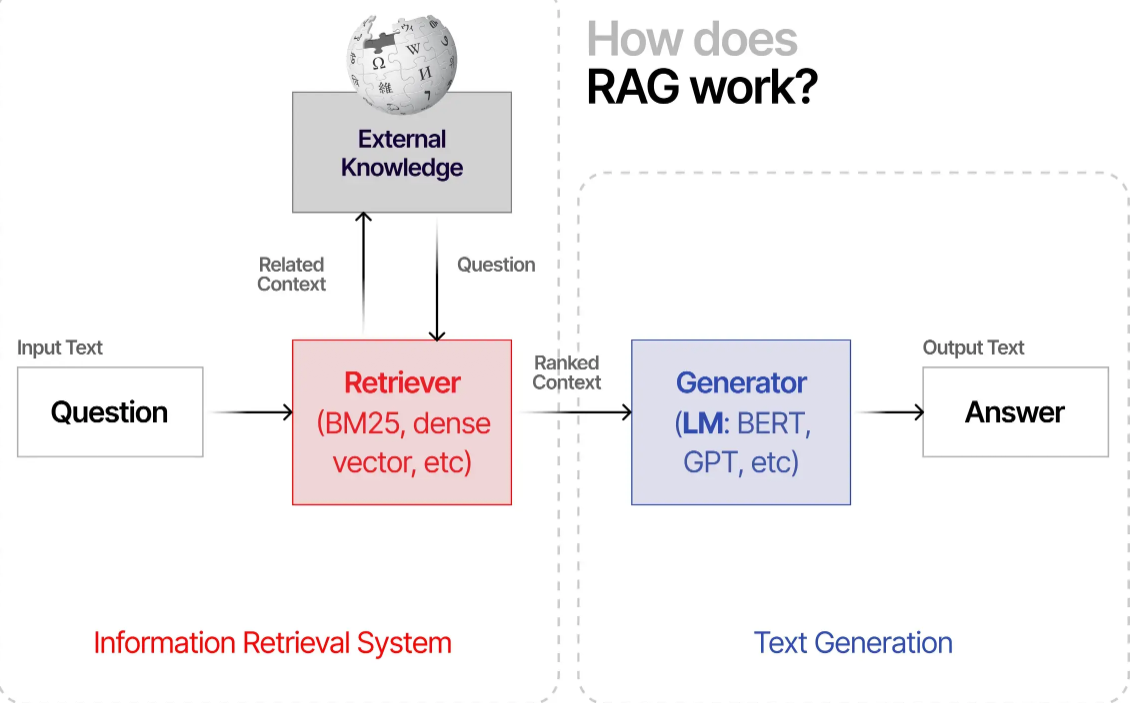
\includegraphics[width=0.9\textwidth]{rag.PNG}
	\caption{RAG system component }\label{fig1}
\end{figure}
As illustrated in Figure 1, the RAG system is built around two main components:the retriever and the generator. The retriever?s role is to find relevant information from a pre-built data store, while the generator utilizes this retrieved data to produce coherent and contextually appropriate content. The overall RAG process operates as follows:
\subsection{Retrieval in RAG Systems}\label{subsec2}

Retrieval is the process of identifying and gathering information system resources that match a specific information need. To break it down, imagine these resources as a key-value store, represented as pairs:

\[
\{(k_i, v_i)\}_{i=1}^{N}
\]

where each key \( k_i \) is linked to a corresponding value \( v_i \) (often, the key and value are the same). When a query \( q \) is provided, the goal is to find the top-\( k \) keys that are most similar to the query using a similarity function \( s \), and then retrieve their associated values.

Depending on the similarity function used, retrieval methods can be grouped into categories such as sparse retrieval, dense retrieval, and others. For the widely used sparse and dense retrieval approaches, the process typically involves two main steps:  \\
1. Encoding each object into a specific representation.\\
2. Building an index to organize the data for efficient searching .

This structured approach ensures that the most relevant information is retrieved quickly and accurately\cite{zhao2024retrievalaugmentedgenerationaigeneratedcontent}.

\subsection{Generator  in RAG Systems}\label{subsec2}
In Retrieval-Augmented Generation (RAG) systems, the generator is a key component responsible for crafting the final output. It works by combining the retrieved information with the users input query to produce a well-structured and contextually relevant response \cite{gupta2024comprehensivesurveyretrievalaugmentedgeneration}.

Once the retriever fetches relevant data from external sources,the generator processes and integrates this information into a well-structured and meaningful answer. At the core of this process is a Large Language Model (LLM), which ensures that the generated text is not only fluent and accurate but also remains relevant to the original query.

In various generative tasks, different models are selected based on the specific requirements: Models like BART\cite{lewis2019bart} and GPT\cite{brown2020language}are commonly used for tasks such as text summarization and translation ,Vision-Language Models (VLMs) \cite{radford2021learningtransferablevisualmodels} are employed to generate textual descriptions from images , for ext-to-Code Generation: Models like OpenAIs Codex \cite{chen2021evaluatinglargelanguagemodels} are designed to translate natural language prompts into executable code.


\section{proposed Slution}\label{sec3}


\section{Experimental Results}\label{sec3}
\subsection{Experiments settings}\label{subsec2}

Equations in \LaTeX\ can either be inline or on-a-line by itself (``display equations''). For
inline equations use the \verb+$...$+ commands. E.g.: The equation
$H\psi = E \psi$ is written via the command \verb+$H \psi = E \psi$+.

For display equations (with auto generated equation numbers)
one can use the equation or align environments:
% KAN Archecture
%\begin{equation}
%f(x_1, x_2, \cdots, x_n)=\sum_{q=1}^{2n+1}\Phi_q %\left( \sum_{p=1}^{n}\phi_{q, p}(x_p)\right)
%\end{equation}

\begin{equation}
\Phi = \{\phi_{p, q}\}, \qquad p=1,2,\cdots, n_{in},\qquad q=1,2,\cdots, n_{out}
\end{equation}

\begin{equation}
x_{l+1,j}=\sum_{i=1}^{n_l}\phi_{l, j, i}(x_{l,i}), \qquad j=1,2,\cdots n_{l+1}
\end{equation}

\begin{equation}
\mathbf{x}_{l+1} = \begin{pmatrix}
\phi_{l,1,1}(\cdot)& \phi_{l,1,2}(\cdot) &\cdots &\phi_{l,1,n_l}(\cdot)  \\
\phi_{l,2,1}(\cdot)&\phi_{l,2,2}(\cdot)  & \cdots &  \phi_{l,2,n_l}(\cdot)\\
\vdots&\vdots  &\ddots  &\vdots  \\
\phi_{l,n_{l+1},1}(\cdot)& \phi_{l,n_{l+1},2}(\cdot) &\cdots  & \phi_{l,n_{l+1},n_l}(\cdot)
\end{pmatrix}\mathbf{x}_{l} =\mathbf{ \Phi}_{l}\mathbf{x}_{l}
\end{equation}
\begin{equation}
\mathbf{KAN(x)}=(\mathbf{\Phi}_{L-1}\circ \mathbf{\Phi}_{L-2}\circ \cdots \circ \mathbf{\Phi}_{1}\circ \mathbf{\Phi}_{0})\mathbf{x}
\end{equation}
% models equations
% system 2
\begin{equation}
y_p(k+1) = f\big[y_p(k), y_p(k-1)\big] + u(k)
\end{equation}
where
\begin{equation*}
f\big[y_p(k), y_p(k-1)\big]=\dfrac{y_p(k)y_p(k-1)[y_p(k)+2.5]}{1+y_p^2(k)+y_p^2(k-1)}
\end{equation*}

% system 3
\begin{equation}
y_p(k+1) = \dfrac{y_p(k)}{1+y_p^2(k)}+ u^3(k)
\end{equation}
% system 4
\begin{equation}
y_p(k+1) = f\big[y_p(k), y_p(k-1), y_p(k-2), u(k), u(k-1)\big] 
\end{equation}
where
\begin{equation*}
f\big[x_1, x_2, x_3,x_4, x_5\big]=\dfrac{x_1x_2x_3x_5(x_3-1)+x_4}{1+x_2^2+x_3^2}
\end{equation*}

\section{Tables}\label{sec5}

Tables can be inserted via the normal table and tabular environment. To put
footnotes inside tables you should use \verb+\footnotetext[]{...}+ tag.
The footnote appears just below the table itself (refer Tables~\ref{tab1} and \ref{tab2}). 
For the corresponding footnotemark use \verb+\footnotemark[...]+

\begin{table}[h]
\caption{Caption text}\label{tab1}%
\begin{tabular}{@{}llll@{}}
\toprule
Column 1 & Column 2  & Column 3 & Column 4\\
\midrule
row 1    & data 1   & data 2  & data 3  \\
row 2    & data 4   & data 5\footnotemark[1]  & data 6  \\
row 3    & data 7   & data 8  & data 9\footnotemark[2]  \\
\botrule
\end{tabular}
\footnotetext{Source: This is an example of table footnote. This is an example of table footnote.}
\footnotetext[1]{Example for a first table footnote. This is an example of table footnote.}
\footnotetext[2]{Example for a second table footnote. This is an example of table footnote.}
\end{table}

\begin{table}[h]
\caption{Example of a lengthy table which is set to full textwidth}\label{tab2}
\begin{tabular*}{\textwidth}{@{\extracolsep\fill}lcccccc}
\toprule%
& \multicolumn{3}{@{}c@{}}{Element 1\footnotemark[1]} & \multicolumn{3}{@{}c@{}}{Element 2\footnotemark[2]} \\\cmidrule{2-4}\cmidrule{5-7}%
Project & Energy & $\sigma_{calc}$ & $\sigma_{expt}$ & Energy & $\sigma_{calc}$ & $\sigma_{expt}$ \\
\midrule
Element 3  & 990 A & 1168 & $1547\pm12$ & 780 A & 1166 & $1239\pm100$\\
Element 4  & 500 A & 961  & $922\pm10$  & 900 A & 1268 & $1092\pm40$\\
\botrule
\end{tabular*}
\footnotetext{Note: This is an example of table footnote. This is an example of table footnote this is an example of table footnote this is an example of~table footnote this is an example of table footnote.}
\footnotetext[1]{Example for a first table footnote.}
\footnotetext[2]{Example for a second table footnote.}
\end{table}

In case of double column layout, tables which do not fit in single column width should be set to full text width. For this, you need to use \verb+\begin{table*}+ \verb+...+ \verb+\end{table*}+ instead of \verb+\begin{table}+ \verb+...+ \verb+\end{table}+ environment. Lengthy tables which do not fit in textwidth should be set as rotated table. For this, you need to use \verb+\begin{sidewaystable}+ \verb+...+ \verb+\end{sidewaystable}+ instead of \verb+\begin{table*}+ \verb+...+ \verb+\end{table*}+ environment. This environment puts tables rotated to single column width. For tables rotated to double column width, use \verb+\begin{sidewaystable*}+ \verb+...+ \verb+\end{sidewaystable*}+.

\begin{sidewaystable}
\caption{Tables which are too long to fit, should be written using the ``sidewaystable'' environment as shown here}\label{tab3}
\begin{tabular*}{\textheight}{@{\extracolsep\fill}lcccccc}
\toprule%
& \multicolumn{3}{@{}c@{}}{Element 1\footnotemark[1]}& \multicolumn{3}{@{}c@{}}{Element\footnotemark[2]} \\\cmidrule{2-4}\cmidrule{5-7}%
Projectile & Energy	& $\sigma_{calc}$ & $\sigma_{expt}$ & Energy & $\sigma_{calc}$ & $\sigma_{expt}$ \\
\midrule
Element 3 & 990 A & 1168 & $1547\pm12$ & 780 A & 1166 & $1239\pm100$ \\
Element 4 & 500 A & 961  & $922\pm10$  & 900 A & 1268 & $1092\pm40$ \\
Element 5 & 990 A & 1168 & $1547\pm12$ & 780 A & 1166 & $1239\pm100$ \\
Element 6 & 500 A & 961  & $922\pm10$  & 900 A & 1268 & $1092\pm40$ \\
\botrule
\end{tabular*}
\footnotetext{Note: This is an example of table footnote this is an example of table footnote this is an example of table footnote this is an example of~table footnote this is an example of table footnote.}
\footnotetext[1]{This is an example of table footnote.}
\end{sidewaystable}

\section{Figures}\label{sec6}

\begin{figure}[h]
\centering

\includegraphics[width=0.9\textwidth]{fig.eps}
\caption{This is a widefig. This is an example of long caption this is an example of long caption  this is an example of long caption this is an example of long caption}\label{fig1}
\end{figure}

In case of double column layout, the above format puts figure captions/images to single column width. To get spanned images, we need to provide \verb+\begin{figure*}+ \verb+...+ \verb+\end{figure*}+.

For sample purpose, we have included the width of images in the optional argument of \verb+\includegraphics+ tag. Please ignore this. 

\section{Algorithms, Program codes and Listings}\label{sec7}

You may refer above listed package documentations for more details before setting \verb+algorithm+ environment. For program codes, the ``verbatim'' package is required and the command to be used is \verb+\begin{verbatim}+ \verb+...+ \verb+\end{verbatim}+. 

Similarly, for \verb+listings+, use the \verb+listings+ package. \verb+\begin{lstlisting}+ \verb+...+ \verb+\end{lstlisting}+ is used to set environments similar to \verb+verbatim+ environment. Refer to the \verb+lstlisting+ package documentation for more details.

A fast exponentiation procedure:

\lstset{texcl=true,basicstyle=\small\sf,commentstyle=\small\rm,mathescape=true,escapeinside={(*}{*)}}
\begin{lstlisting}
begin
  for $i:=1$ to $10$ step $1$ do
      expt($2,i$);  
      newline() od                (*\textrm{Comments will be set flush to the right margin}*)
where
proc expt($x,n$) $\equiv$
  $z:=1$;
  do if $n=0$ then exit fi;
     do if odd($n$) then exit fi;                 
        comment: (*\textrm{This is a comment statement;}*)
        $n:=n/2$; $x:=x*x$ od;
     { $n>0$ };
     $n:=n-1$; $z:=z*x$ od;
  print($z$). 
end
\end{lstlisting}

\begin{algorithm}
\caption{Calculate $y = x^n$}\label{algo1}
\begin{algorithmic}[1]
\Require $n \geq 0 \vee x \neq 0$
\Ensure $y = x^n$ 
\State $y \Leftarrow 1$
\If{$n < 0$}\label{algln2}
        \State $X \Leftarrow 1 / x$
        \State $N \Leftarrow -n$
\Else
        \State $X \Leftarrow x$
        \State $N \Leftarrow n$
\EndIf
\While{$N \neq 0$}
        \If{$N$ is even}
            \State $X \Leftarrow X \times X$
            \State $N \Leftarrow N / 2$
        \Else[$N$ is odd]
            \State $y \Leftarrow y \times X$
            \State $N \Leftarrow N - 1$
        \EndIf
\EndWhile
\end{algorithmic}
\end{algorithm}

%%=============================================%%
%% For presentation purpose, we have included  %%
%% \bigskip command. Please ignore this.       %%
%%=============================================%%
\bigskip
\begin{minipage}{\hsize}%
\lstset{frame=single,framexleftmargin=-1pt,framexrightmargin=-17pt,framesep=12pt,linewidth=0.98\textwidth,language=pascal}% Set your language (you can change the language for each code-block optionally)
%%% Start your code-block
\begin{lstlisting}
for i:=maxint to 0 do
begin
{ do nothing }
end;
Write('Case insensitive ');
Write('Pascal keywords.');
\end{lstlisting}
\end{minipage}

\section{Cross referencing}\label{sec8}

%Environments such as figure, table, equation and align can have a label
%declared via the \verb+\label{#label}+ command. For figures and table
%environments use the \verb+\label{}+ command inside or just
%below the \verb+\caption{}+ command. You can then use the
%\verb+\ref{#label}+ command to cross-reference them. As an example, consider
%the label declared for Figure~\ref{fig1} which is
%\verb+\label{fig1}+. To cross-reference it, use the command 
%\verb+Figure \ref{fig1}+, for which it comes up as
%``Figure~\ref{fig1}''. 

To reference line numbers in an algorithm, consider the label declared for the line number 2 of Algorithm~\ref{algo1} is \verb+\label{algln2}+. To cross-reference it, use the command \verb+\ref{algln2}+ for which it comes up as line~\ref{algln2} of Algorithm~\ref{algo1}.

\subsection{Details on reference citations}\label{subsec7}

Standard \LaTeX\ permits only numerical citations. To support both numerical and author-year citations this template uses \verb+natbib+ \LaTeX\ package. For style guidance please refer to the template user manual.

%Here is an example for \verb+\cite{...}+: \cite{bib1}. Another example for %\verb+\citep{...}+: \citep{bib2}. For author-year citation mode, \verb+\cite{...}+ %prints Jones et al. (1990) and \verb+\citep{...}+ prints (Jones et al., 1990).

%All cited bib entries are printed at the end of this article: \cite{bib3}, %\cite{bib4}, \cite{bib5}, \cite{bib6}, \cite{bib7}, \cite{bib8}, \cite{bib9}, %\cite{bib10}, \cite{bib11}, \cite{bib12} and \cite{bib13}.


\section{Examples for theorem like environments}\label{sec10}

For theorem like environments, we require \verb+amsthm+ package. There are three types of predefined theorem styles exists---\verb+thmstyleone+, \verb+thmstyletwo+ and \verb+thmstylethree+ 

%%=============================================%%
%% For presentation purpose, we have included  %%
%% \bigskip command. Please ignore this.       %%
%%=============================================%%
\bigskip
\begin{tabular}{|l|p{19pc}|}
\hline
\verb+thmstyleone+ & Numbered, theorem head in bold font and theorem text in italic style \\\hline
\verb+thmstyletwo+ & Numbered, theorem head in roman font and theorem text in italic style \\\hline
\verb+thmstylethree+ & Numbered, theorem head in bold font and theorem text in roman style \\\hline
\end{tabular}


\section{Discussion}\label{sec12}

Discussions should be brief and focused. In some disciplines use of Discussion or `Conclusion' is interchangeable. It is not mandatory to use both. Some journals prefer a section `Results and Discussion' followed by a section `Conclusion'. Please refer to Journal-level guidance for any specific requirements. 

\section{Conclusion}\label{sec13}

Conclusions may be used to restate your hypothesis or research question, restate your major findings, explain the relevance and the added value of your work, highlight any limitations of your study, describe future directions for research and recommendations. 

In some disciplines use of Discussion or 'Conclusion' is interchangeable. It is not mandatory to use both. Please refer to Journal-level guidance for any specific requirements. 

\backmatter

\bmhead{Supplementary information}

If your article has accompanying supplementary file/s please state so here. 

Authors reporting data from electrophoretic gels and blots should supply the full unprocessed scans for key as part of their Supplementary information. This may be requested by the editorial team/s if it is missing.

Please refer to Journal-level guidance for any specific requirements.

\bmhead{Acknowledgements}

Acknowledgements are not compulsory. Where included they should be brief. Grant or contribution numbers may be acknowledged.

Please refer to Journal-level guidance for any specific requirements.

\section*{Declarations}

Some journals require declarations to be submitted in a standardised format. Please check the Instructions for Authors of the journal to which you are submitting to see if you need to complete this section. If yes, your manuscript must contain the following sections under the heading `Declarations':

\begin{itemize}
\item Funding
\item Conflict of interest/Competing interests (check journal-specific guidelines for which heading to use)
\item Ethics approval and consent to participate
\item Consent for publication
\item Data availability 
\item Materials availability
\item Code availability 
\item Author contribution
\end{itemize}

%%===================================================%%
%% For presentation purpose, we have included        %%
%% \bigskip command. Please ignore this.             %%
%%===================================================%%


%%===========================================================================================%%
%% If you are submitting to one of the Nature Portfolio journals, using the eJP submission   %%
%% system, please include the references within the manuscript file itself. You may do this  %%
%% by copying the reference list from your .bbl file, paste it into the main manuscript .tex %%
%% file, and delete the associated \verb+\bibliography+ commands.                            %%
%%===========================================================================================%%

\bibliography{sn-bibliography}% common bib file
%% if required, the content of .bbl file can be included here once bbl is generated
%%\input sn-article.bbl


\end{document}
